\livelloA{Probability}

\begin{frame}
  \vspace*{.5cm}
  The mathematical statistics is different from the applied statistics. It builds probability models.\\
  \vspace*{.5cm}
  In statistics the aim is to associate the examined sample with a model. This connection is never clear and conclusive because an infinite number of data is not available: the connection between the data and a model is an asymptotic process.\\
  \vspace*{.5cm}
  It is easier to create models for centrality and variability indexes than for extreme percentiles, because the second ones are more sensitive to little variations.
\end{frame}

\begin{frame}
  The nature of the concept of probability, in an empirical sense, can be stated like follows: \\
  \textbf{In a sequence of trials, done in the same conditions, the frequency of an event comes nearer to the probability of the same event. The approximations tends to ameliorate when the number of trials increases.}\\
  \vspace*{.2cm}
  With the same number of possible cases, the probability of an event increases when the number of favourable cases increases. It can also happen when, with the same number of favourable cases, the number of possible cases decreases. \\
  \vspace*{.2cm}
  The first (in the historical sense) \textbf{definition of classic probability:}\\
  \textbf{The probability of a random event is the ratio between the number of favourable cases and the number of possible cases, as long as they have the same probability.}\\
\end{frame}

\begin{frame}
  The concept of \textbf{classic probability}, founded on a \textbf{mathematical probability} or \textbf{prior}, has been the first one to be defined.\\
  \vspace*{.25cm}
  It is the probability to obtain heads or tails with a coin, to have a number from 1 to 6 with a dice or in more throwings, to foresee the arrival orders in a competition with various contestants who respect the previous four conditions.\\
  \vspace*{.25cm}
  No experimental datum is required. The results are prior known, and it is not necessary to wait for gatherings or observations. \textbf{It is only necessary the logic reasoning in order to accurately calculate the probability}.\\
  \vspace*{.25cm}
  If the coin, the dice or the match are not loaded, the experimental tests will leave the expected data only for negligible quantities, determined by random events or observational errors.
\end{frame}

\begin{frame}
  The estimation of a \textbf{prior probability} has serious restrictions in the experimental reasearch. In order to calculate the probability of an event, it is necessary to previously know the various probabilities of all the possible events.\\
  \vspace*{.25cm}
  \textbf{For this reason, this approach cannot be always used.}\\
  \vspace*{.25cm}
  As estimation of the \textbf{probability of an experimental event} it can be used its \textbf{frequency}.\\
  \vspace*{.2cm}
  The probability of a random event is the limit to which it tends when the number of observations increases, in a series of experiences recurring in the same conditions.
  $$ P = \lim_{n\rightarrow\infty}{f} $$\\
  It also exists another kind of probability called \textit{\textbf{posterior probability}}. This is not a topic of this course. 
\end{frame}

\begin{frame}
  \vspace*{.25cm}
  If {\boldmath $ F $} is the relative frequence of an event in a population, it is generally possible to observe that, when the number of observations ({\boldmath $ n $}) increases, the  frequency ({\boldmath $ f $}) of the sample tends to become similar to the real one or to that of the population ({\boldmath $ F $}).\\
  \vspace*{.25cm}
  This statement cannot be proved either with mathematical instruments, because it refers to osbervational data, or in an empirical way, because, in the reality, it is not possible to repeat an experiment infinite times.\\
  \vspace*{.25cm}
  Anyway, it is a \textbf{statistical regularity}, called \textbf{law of large numbers}, that is the experimental basis both of every statistics theory and of mathematical reasoning.
\end{frame}

\begin{frame}
  \vspace*{.25cm}
  In these cases, it is a matter of \textbf{frequentist probability}, of a \textbf{posterior probability}, of \textbf{law of large numbers}, or of \textbf{statistical probability}.\\
  \vspace*{.4cm}
  \textbf{It is possible to answer to a lot of empirical questions in only one way:} \\
  \vspace*{.2cm}
  \textbf{To conceive a series of observations or experimentations, in unrelieved or statistically checked conditions, in order to point out the frequency.}
\end{frame}



\livelloA{Discrete and continuous distributions}

\begin{frame}
  Irrespective of the probability is empirical or mathematical, there are some \textbf{probability distributions} able to explain the phenomenon.
  \begin{center}
    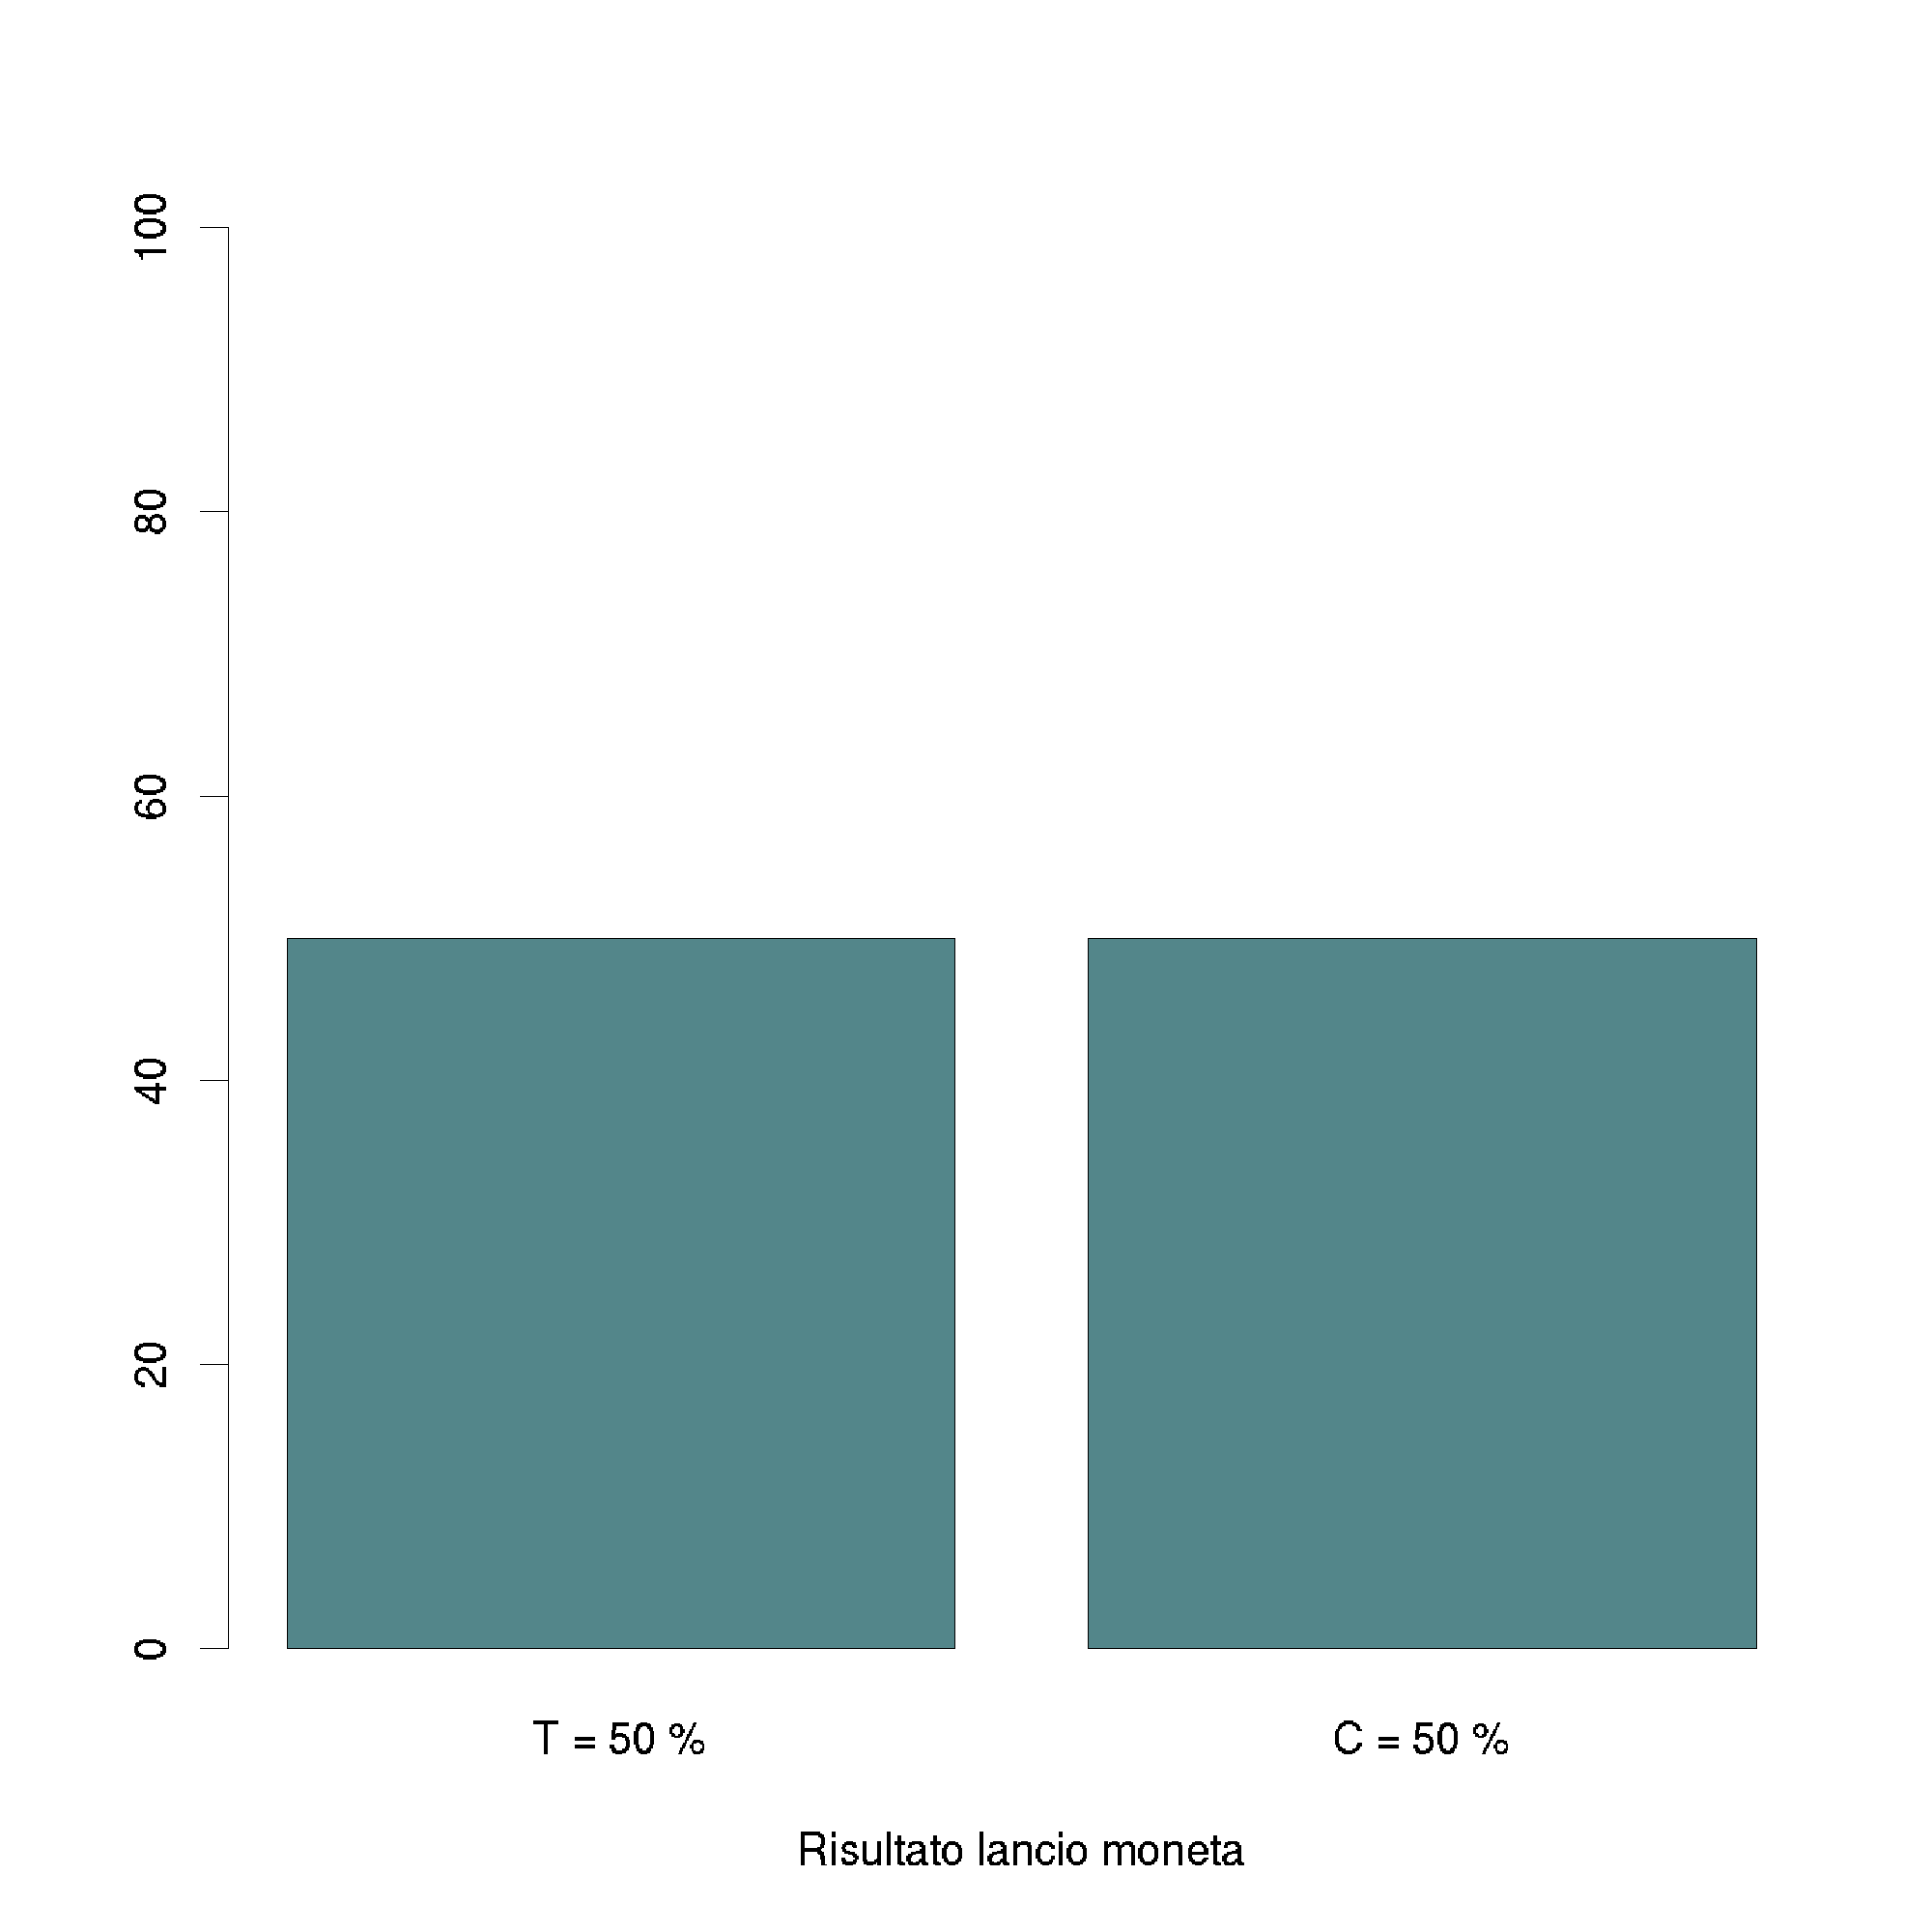
\includegraphics[scale=0.6]{g1.png}
  \end{center}
  The chart represents a discrete variables distribution. It is a mathematical representation that deals with data. 
\end{frame}

\begin{frame}
  Numerical outcomes for a random phenomenon can be described by mathematical instruments called \textbf{random variables} (or \textbf{unpredictable}).\\
  \vspace*{.2cm}
  Random variables are ``mathematical models'' which gives probability values to possible numerical values. Their corresponding \textbf{probability distributions can be of two kinds: discrete or continuous.}\\
  \vspace*{.2cm}
  In the \textbf{discrete random variables}, the argument values are the natural numbers: 0, 1, 2, \dots, $ n $. They are necessary to calculate the probability of events that have a discrete number (finite or infinite) of recurrences.\\
  \vspace*{.2cm}
  A \textbf{random variable} is \textbf{continuous} when its distribution is continuous. With this continuous variable, it is estimated the probability to extract not a single value but equal or greater values (or equal or less values).\\
  The probabilities are calculated only for intervals values in the case of continuous random varibales. For specific values, they are always zero.
\end{frame}



\livelloA{Discrete distributions}

\begin{frame}
  Among the discrete distribution, two are really important in statistics for their quality:\\
  \begin{itemize}
    \item Binomial
    \item Poisson
  \end{itemize}
  Both the distributions explain phenomenon related to the behavior of binary phenomenon: error - success, goes - does not goes, \\defective - not defective.\\
  \vspace*{.2cm}
  In particular, they define the number of successes that can be verified in $ N $ trials, given a certain probability of success of each trial.\\
  \vspace*{.2cm}
  The two functions are different because:
  \begin{itemize}
    \item the Binomial deals with medium-high probability events;
    \item the Poisson deals with very low probability events.
  \end{itemize}
\end{frame}

\livelloB{Binomial distribution}

\begin{frame}
  \vspace*{.3cm}
  The \textbf{binomial is a discrete and finite theoretical distribution}, for events classified with a \textbf{binary variable} and it is defined by the following density function:\\
  \vspace*{.3cm}
  $$ p_n(x) = \frac{n!}{x!(n-x)!} \, p^x(1-p)^{n-x} $$
  \begin{tabbing}
    where: \hspace*{.25cm} \= \\
    \hspace*{.1cm} \> $ x $ = number of successes \\
    \hspace*{.1cm} \> $ p $ = probability of success of a single trial \\
    \hspace*{.1cm} \> $ n $ = number of trials
  \end{tabbing}
\end{frame}

\begin{frame}
  \vspace*{.5cm}
  For example, if the {\boldmath $ p $} parameter is the probability of the event ``throwing a coin it gives heads'', and then $ p = 0.5 $, it is possible to calculate the probability that on {\boldmath $ n $}=10 throwings, the number of successes {\boldmath $ x $} is equal to 8:\\
  \vspace*{.5cm}
  $$ P_{10}(8) = \frac{10!}{8!\cdot 2!}\cdot 0.5^8 \cdot 0.5^2 = 0.04 \rightarrow 4 \% $$  
\end{frame}

\begin{frame}
  The probability distribution of the binomial depends on 2 parameters: {\boldmath $ p $} and {\boldmath $ n $}.\\
  \vspace*{.2cm}
  If $ p $ and {\boldmath $ q = 1-p $} are equal to 0.5 the distribution is always symmetric, independently of $ n $. If $ p $ is highly greater or less than $ q $, the distribution is asymmetric. This asymmetry tends to decrease when $ n $ increases.\\
  \vspace*{.2cm}
  The binomial distribution is usually used for $ p $ values that go from 0.1 to 0.9. For $ p $ values excluded from this interval, the Poisson distribution is used when $ n $ is not high.\\
  \vspace*{.2cm}
  When $ n $ is so high that even the result of {\boldmath$n \cdot p$} is high, the binomial one is used, for each value of $ p $.\\
  \vspace*{.2cm}
  When a sample has big dimensions, the probabilities estimation can be obtained by the normal distribution.
\end{frame}

\livelloB{Poisson distribution}

\begin{frame}
  \vspace*{.25cm}
  When the number of data $ n $ is really high and the probability $ p $ is really small, the binomial distribution has some practice disadvantages. They were really important before the introduction of the automatic calculation: to raise really small frequencies to high powers and the calculation of factors for high numbers, make the manual calculation almost impossible.\\
  \vspace*{.25cm}
  \textbf{For {\boldmath $ n $} that tends to infinite and {\boldmath $ p $} that tends to 0, in a way that $n \cdot p$ is constant, Poisson demonstrated that}:\\
  \vspace*{.25cm}
  $$ P_i = \frac{\mu^i}{i!}\, e^{-\mu} $$\\
  \vspace*{.5cm}
  \textbf{if:} \hspace{1 cm} $n\rightarrow \infty$ \hspace{1 cm} $p\rightarrow 0$ \hspace{1 cm} $n \cdot p = \mu$
\end{frame}

\begin{frame}
  \vspace*{.25cm}
  \textbf{The Poisson is a discrete theoretical distribution and it is totally defined by only one parameter, the mean {\boldmath $ \mu $}}.\\
  \vspace*{.5cm}
  Even in the Poisson distribution, the {\boldmath $ \mu $} expected mean is given by {\boldmath $n \cdot p $}.\\ 
  \vspace*{.5cm}
  So that the frequencies or probabilities calculated with the Poisson law are exact, $\mu$ must be a constant parameter for the whole distribution.\\
  \vspace*{.5cm}
  Also in this distribution {\boldmath $ \; \sigma^2 = n \cdot p \cdot q $}.\\
\end{frame}

\begin{frame}
  \vspace*{.25cm}
  It is possible to easily verify that the variance is equal to the mean: if we use the just illustrated three conditions, the Poisson distribution variance will be given by:
  \vspace*{.25cm}
  $$ \sigma^2 = \lim_{\substack{n \rightarrow \infty \\ p \rightarrow 0}}{(n \cdot p \cdot q)} = \lim_{\substack{n \rightarrow \infty \\ p \rightarrow 0}}{(n \cdot p) \cdot q} = \lim_{\substack{n \rightarrow \infty \\ p \rightarrow 0}}{\; k \cdot (1- p)} = k = \mu $$\\
  \begin{center}
    Or rather \textbf{if {\boldmath $ p $} tends to 0, {\boldmath $ q $} tends to 1; and then {\boldmath $ \;n \cdot p = n \cdot p \cdot q $}.}
  \end{center}
  \vspace*{.35cm}
  The Poisson distribution law is also called \textbf{law of rare events}, because the probability that the event happens is really low.\\
  \vspace*{.25cm}
  It is also called \textbf{law of small numbers}, because the absolute frequency of these events is expressed by a small number, even in an high number of trials.
\end{frame}

\begin{frame}
  \vspace*{.5cm}
  The Poisson distribution has a very asymmetric shape and the most frequent and probable class is zero, when $ \mu $ is less than 1. It is still asymmetric for values of $ \mu $ less than 3.\\
  \vspace*{.5cm}
  A mean equal to 6-7 establishes a symmetric distribution of probabilities and it is well approximated by the normal (or Gaussian) distribution.
\end{frame}

\begin{frame}
  \vspace*{.25cm}
  The Poisson distribution can be used instead of the binomial one, for $ p $ less than 0.05 and $ n $ greater than 100.\\
  \vspace*{.5cm}
  The Poisson distribution is used for events that happen both in the space and in the time. For example, the number of not wanted particles in a little space or the number of events that can happen in a little time.\\
  \vspace*{.5cm}
  In a great number of books, the mean number of events is not shown with $ \mu $ but with {\boldmath $ \lambda $}, particularly when it deals with temporal events.\\
  \vspace*{.5cm}
  In order to have the Poisson distribution, a random variable must have \textbf{three requirements: stationarity, not-multiplicity, independence}.
\end{frame}

\begin{frame}
  \vspace*{.25cm}
  A random variable :
  \begin{itemize}
    \item is \textbf{stationary}, when the probability of each event in a time interval ({\boldmath $ t, t + h $}) or in an infinitesimal space is approximately constant, equal to {\boldmath $ \lambda h $} for each $ t $.
    \item It has the \textbf{not-multiplicity} requirement, when the probability that two or more events happen in the same infinitesimal time or space interval $ \lambda h $ is highly smaller than in the case of only one event. This means that the probability to have two or more events is highly smaller than to have only one event;
    \item is \textbf{independent} if, in an interval and in a finite space, the events are independent one from the others and the number of events that happened in an interval is independent from that of the others.
  \end{itemize}
\end{frame}

\begin{frame}
  \vspace*{.25cm}
  As the chart highlights, the probabilities distribution with mean($ \mu $) 0.9 is highly asymmetric, with right asymmetry. \\
  \vspace*{.5cm}
  \begin{figure}
    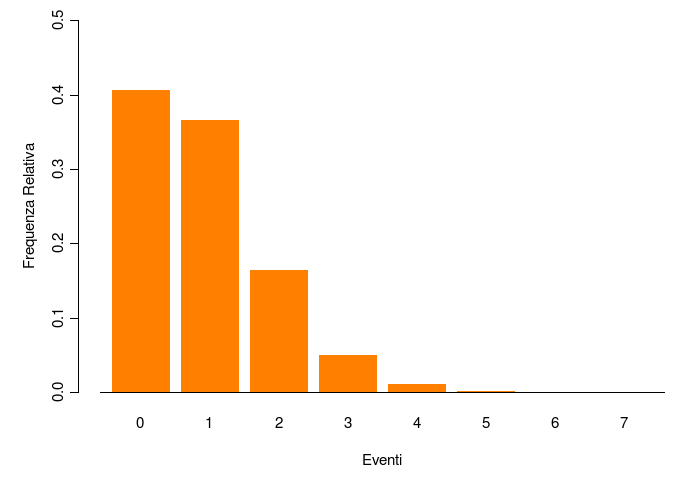
\includegraphics[scale=0.3]{2_18.png}
  \end{figure}
\end{frame}

\begin{frame}
  \vspace*{.25cm}
  The probabilities distribution with $ \mu = 12 $ has an ``almost normal'' shape: the higher probabilities regard the events around the mean 12. \\
  \vspace*{.25cm}
  \begin{floatingfigure}[l]{6.5cm}
    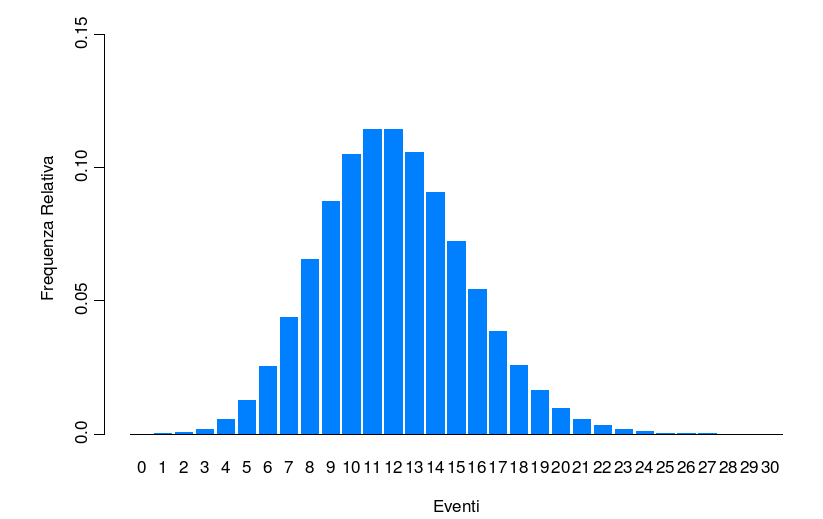
\includegraphics[scale=0.3]{2_19.png} 
  \end{floatingfigure}
  \hspace*{.25cm}\\
  Around 12, the probabilities decrease in an almost asymmetric way, with differences from the normal distribution that can be ignored, as shown in the graphic.
\end{frame}

\begin{frame}
  \begin{small}
    It is supposed to throw two dices with twelve faces for $ N $ times and to sum the result of the two dices.\\
    \vspace*{.2cm}
    We repeat the experiments for $ P $ times.\\
    \vspace*{.2cm}
    Each of the $ P $ times we write down how many times the sum is equal to two and to thirteen.\\
    \vspace*{.2cm}
    \centering
    \textbf{Example: Poisson and Binomial simulations}\\              
  \end{small}
  \begin{figure}
    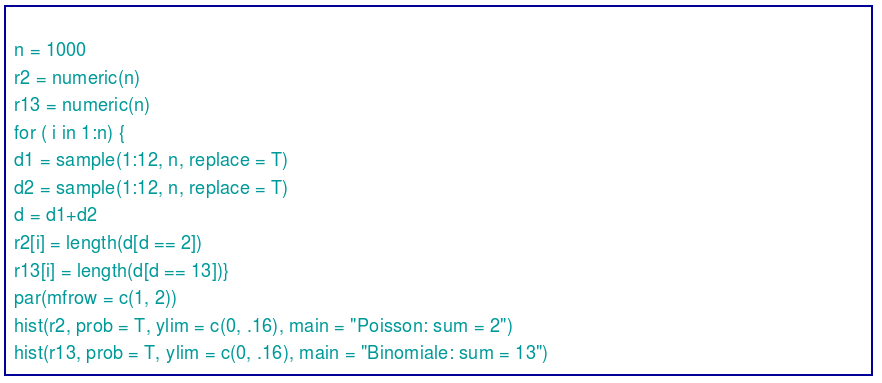
\includegraphics[scale=0.29]{2_20.png}
  \end{figure}
\end{frame}



\livelloA{Continuous distributions}

\begin{frame}
  \vspace*{.5cm}
  All the previous models give the theoretical distribution of discrete random variables. When it is necessary to describe \textbf{continuous and positive random variables}, as measurements or time, the most useful models are the ones that follow.\\
  \vspace*{.5cm}
  Among them, the most frequent distribution and the most useful one for the experimental research, which is the \textbf{basis of the parametric statistics}, is the \textbf{normal or Gaussian distribution}.
\end{frame}

\livelloB{Normal distribution}

\begin{frame}
  \vspace*{.5cm}
  The most important continuous distribution is the normal curve.\\
  \vspace*{.5cm}
  The name \textbf{normal curve} comes from the convinction (not always correct) that a great number of phenomenon, both the biological ones and the physical one, are usually distributed according the \textbf{Gaussian curve}.\\
  \vspace*{.5cm}
  Its name \textbf{curve of accidental errors}, mainly spread in the phisical subjects, comes from the experimental observations where the distribution of errors, committed when the same size is measured many times, results to be well approximated by this curve.
\end{frame}

\begin{frame}
  \vspace*{.5cm}
  The normal distribution is defined by two parameters:
  \begin{itemize}
    \item $ \mu $, location parameter, that establishes the position of the distribution;
    \item $ \sigma $, scale parameter, that establishes the size of the distribution.
  \end{itemize}
  \vspace*{.75cm}
  It is defined from $ -\infty $ to $ +\infty $, and, as it is a probability distribution, its integral from $ -\infty $ to $ +\infty $ is equal to 1.\\
  \vspace*{.75cm}
  At the extremes, it asymptotically tends to zero, and in the tails over the value $6\sigma$, the area underlying is so limited that, with a good approximation, can be considered cut off.
\end{frame}

\begin{frame}
  \vspace*{.5cm}
  From the theoretical point of view, the normal distribution well represents observational errors, the noise and other phenomenon using a mathematical model.\\
  \vspace*{.75cm}
  The \textbf{probability} that the variable has a value between two specific values, corresponds to the measure of the area underlying the curve included between the two values (the area represented in the following picture).\\
  \vspace*{.75cm}
  The probability that the variable as a precise value is equal to zero, as the area (integral) included between the value and itself is null (the segment represented in the picture).
\end{frame}

\begin{frame}
  \begin{center}
    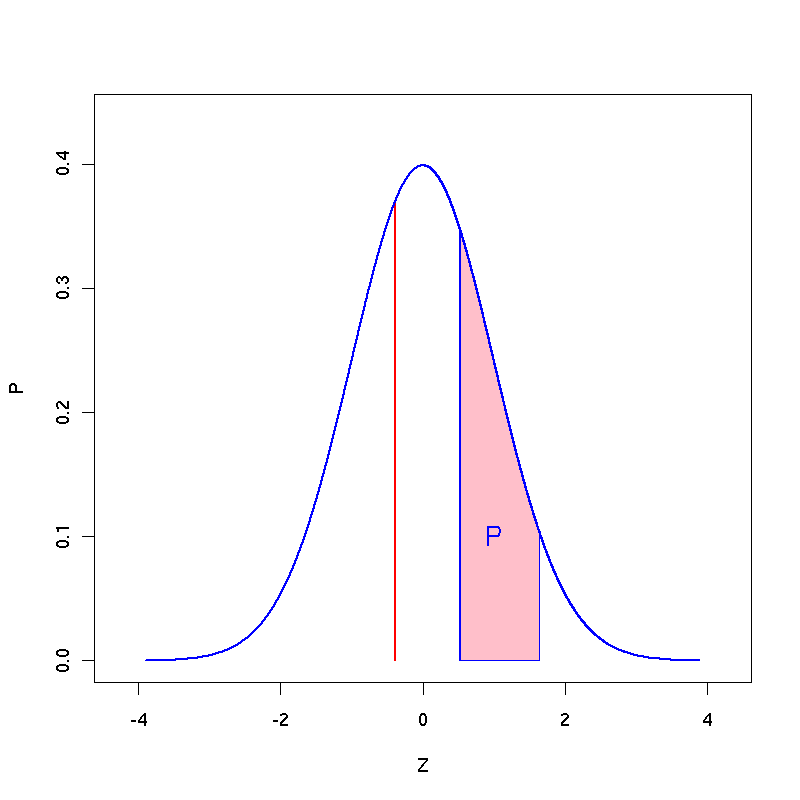
\includegraphics[scale=0.3]{g2.png}
  \end{center}
\end{frame}

\begin{frame}
  \vspace*{.25cm}
  From the mathematical point of view, the Gaussian distribution can be considered as the limit of the binomial distribution:\\
  \begin{itemize}
    \item for $ n $ that tends to infinite;
    \item while both $ p $ and $ q $ don't tend to 0 (this condition distringuishes the Gaussian distribution from the Poisson one).
  \end{itemize}
  \vspace*{.25cm}
  If $ n $ tends to infinite and $ p $ stays constant, the mean ($ n \cdot p $) is approximated to infinite and makes the distribution without any practice applications.\\
  \vspace*{.25cm}
  On the contrary, the considered variable, that with few data was qualified by discrete unities, can be expressed by always smaller unities. It will become acceptable to define it as a continuous quantity.\\
  The Gaussian distribution can be considered also the limit of the Poisson distribution, when $ i $ e $ \mu $ become really high.
\end{frame}

\begin{frame}
  \vspace*{.25cm}
  The mathematical formula of the normal distribution is the following one:
  \vspace*{.25cm}
  $$ y = f(x) = N(\mu,\sigma) = \frac{1}{\sigma \sqrt{2\pi}}\, e^{-\frac{1}{2} \left( \frac{x-\mu}{\sigma} \right) ^2} $$ \\
  \vspace*{.25cm}
  that is the expression of the \textbf{probability density function} (or relative frequencies function) of the normal distribution.\\
  \vspace*{.25cm}
  In less mathematical words, \textbf{it allows to estimate the $ y $ value (the value of the y-axis or the height of the curve) for each $ x $ value (the x-axis value)}.\\
  \vspace*{.25cm}
  The $ \mu $ and $ \sigma $ values completely define the normal density function.\\
  \vspace*{.25cm}
  \textbf{Infinite normal density curve exist}.
\end{frame}

\begin{frame}
\vspace*{.25cm}
This is the graphical representation of a Normal.\\
\vspace*{.25cm}
\begin{figure}
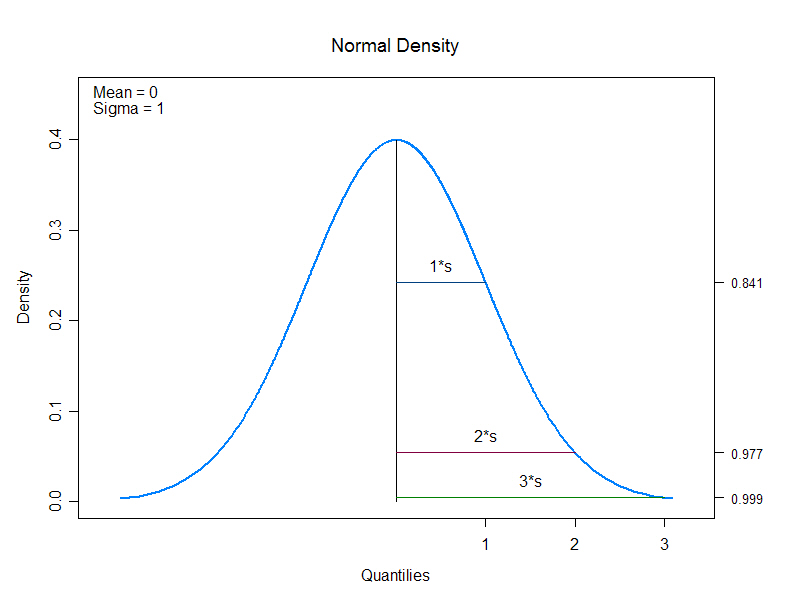
\includegraphics[scale=0.3]{2_25.png}
\end{figure}
\end{frame}

\begin{frame}
  \vspace*{.25cm}
  The most important characteristics of the normal distribution are: a relatively higher frequencies of the central values and gradually lower frequencies towards the extremes. \\
  \vspace*{.25cm}
  The density function is symmetric compared to/around the mean: it increases from $ -\infty $ to the mean and then it decreases up to $ +\infty $. \\
  \vspace*{.25cm}
  It has two inflection points: the first one, rising, in the point $ \mu - \sigma $; the second one, descending, in the point $ \mu + \sigma $. \\
  \vspace*{.25cm}
  In every normal curve, the mean, the mode and the median coincide. \\
  \vspace*{.25cm}
  \textbf{If the distribution is normal, in order to know its distribution, it is enough to know two parameters of a series of data, the mean {\boldmath$ \mu $} and the variance {\boldmath$ \sigma ^2 $}}.
\end{frame}

\begin{frame}
  \vspace*{.25cm}
  If $ \mu $ changes and $ \sigma $ stays constant, the result is an infinite number of normal curves with the same shape and dimension, but with the symmetric axis in a different point.
  \begin{figure}
    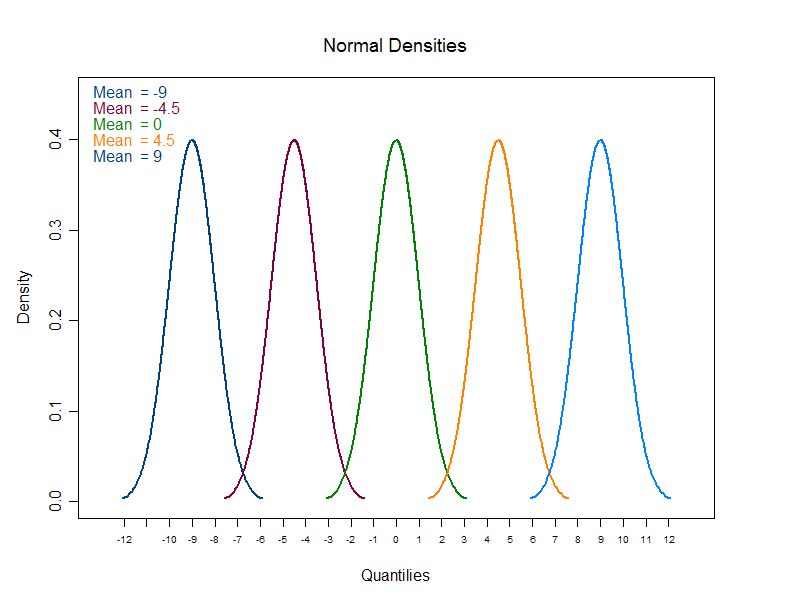
\includegraphics[scale=0.3]{2_27.png}
  \end{figure}
\end{frame}

\begin{frame}
  \vspace*{.25cm}
  If, on the contrary, $ \mu $ stays constant and $ \sigma $ changes, all the infinite curves have the same symmetric axis; but they are almost flat, according to the $ \sigma $ value.
  \begin{figure}
    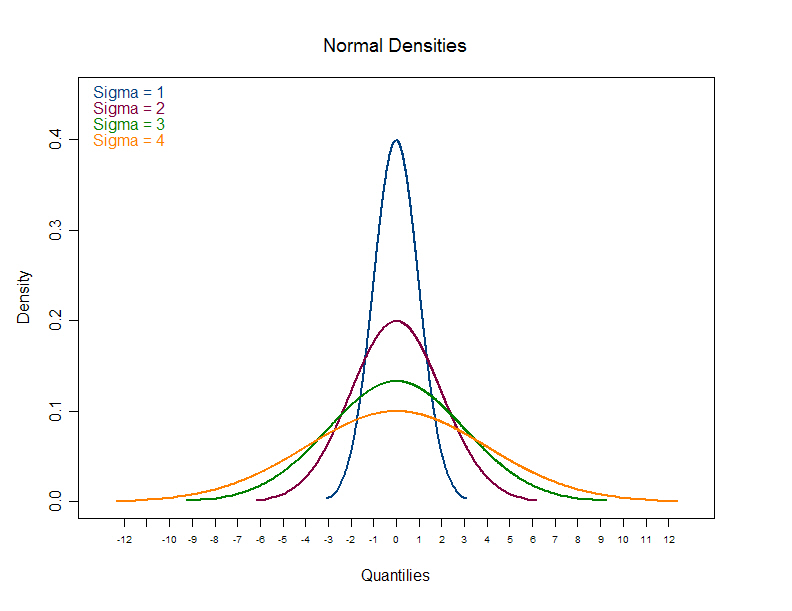
\includegraphics[scale=0.3]{2_28.png}
  \end{figure}
\end{frame}

\begin{frame}
  \vspace*{.25cm}
  These are two normal distributions which are different both for their mean ($ \mu $) and for the dispersion of data ($ \sigma $).
  \begin{figure}
    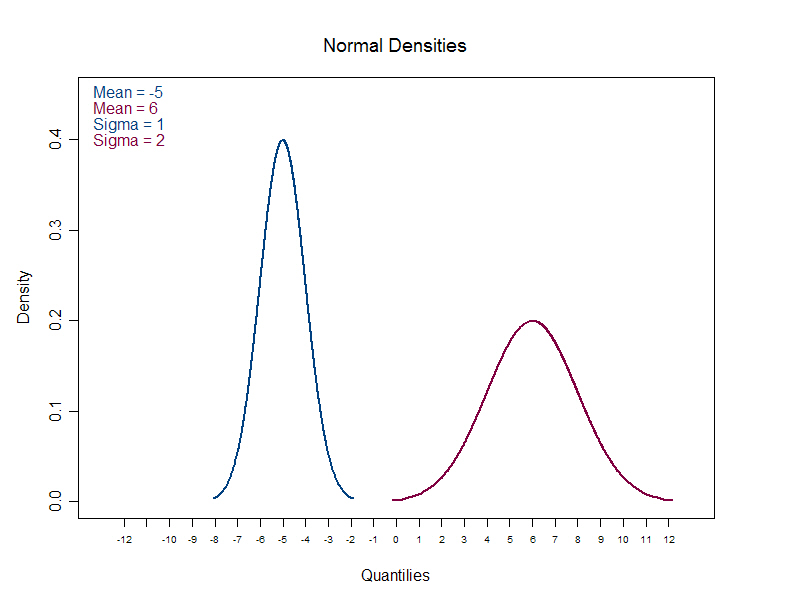
\includegraphics[scale=0.3]{2_29.png}
  \end{figure}
\end{frame}

\livelloB{Standard normal distribution}

\begin{frame}
  The infinite shapes of the normal distribution, determined by the combination of the differences of the mean and the variance, can be all connected to the same shape.\\
  \vspace*{.25cm}
  It is the \textbf{standard normal distribution} or \textbf{reduced normal}, which is obtained by the transformation of the variable given by:
  \vspace*{.25cm}
  $$ Z = \frac{X-\mu} {\sigma} $$
  \vspace*{.25cm}
  The \textbf{standardizing} is a transformation that consists in:
  \begin{itemize}
    \item making the mean equal to zero ($ \mu = 0 $), because the mean is subtracted to every value;
    \item taking the standard deviation ($ \sigma $) as unit of measurement ($ \sigma = 1 $) of the new variable.
  \end{itemize}
\end{frame}

\begin{frame}
  \vspace*{.5cm}
  After the change of the variable, in the reduced normal, the probability density is given by:\\
  \vspace*{.25cm}
  $$y = f(z) = N(0,1) = \frac{1}{\sqrt{2\pi}}\,e^{-\frac{1}{2}z^2} $$\\
  \vspace*{1cm}
  This formula highlights how \textbf{the distribution's shape does not depend either on the mean or on the variance of the original distribution}.
\end{frame}

\begin{frame}
  \begin{figure}
    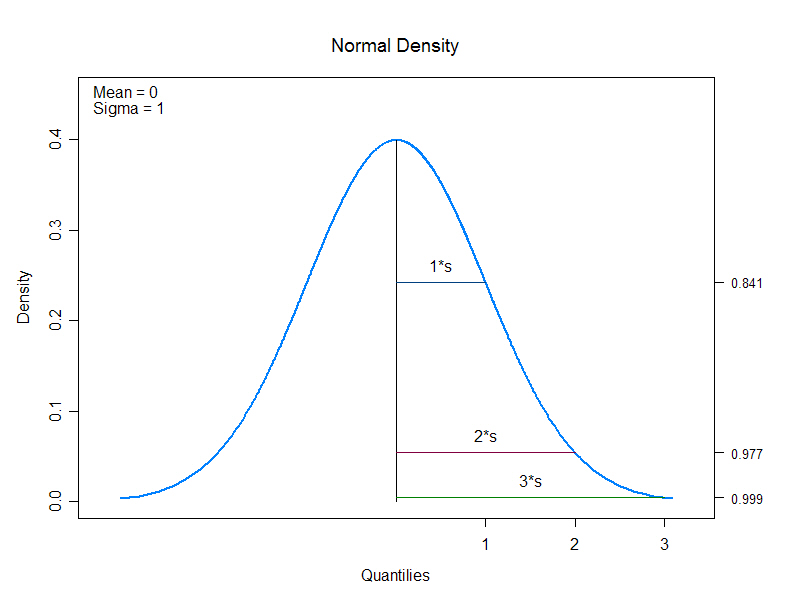
\includegraphics[scale=0.35]{2_32.png}
  \end{figure}
\end{frame}

\livelloB{Characteristics of the normal distribution}

\begin{frame}
  \begin{small}
    \vspace*{.2cm}
    In the statistics practice, \textbf{the most useful characteristics of the normal distribution} are not the ratio between x-axis and y-axis, explained before, \textbf{but the relations between the distance from the mean and the probability density represented by the curve}.\\
    \vspace*{.2cm}
    In an easiest way, it is possible to define how many data are included between the mean and a specific value. This is obtained by measuring the distance from the {\boldmath$\mu$} mean in {\boldmath$\sigma$} standard deviations unities.\\
    \vspace*{.2cm}
    The fraction of the cases included:
    \begin{itemize}
      \item between $ \mu + \sigma $ and $ \mu - \sigma $ is equal to 68.27\%;
      \item that between $ \mu + 2 \sigma $ and $ \mu - 2 \sigma $ is equal to 95.45\%;
      \item that between $ \mu + 3 \sigma $ and $ \mu - 3 \sigma $ is equal to 99.73\%.
    \end{itemize}
    \vspace*{.2cm}
    In pratice, in the normal curve, almost all the data are included around the mean whose wideness is {\boldmath $ 3\sigma $}.
  \end{small}
\end{frame}

\begin{frame}
  \vspace*{.5cm}
  \begin{floatingfigure}[r]{8.5cm}
    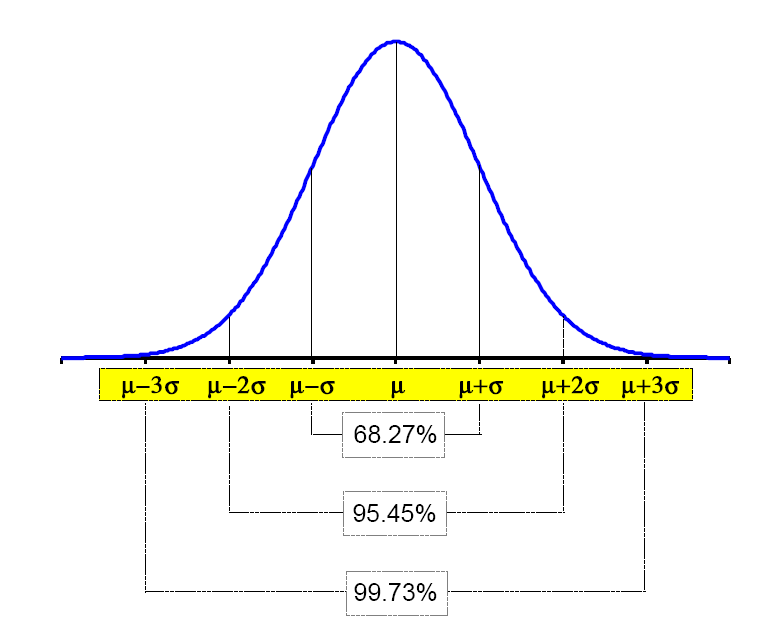
\includegraphics[scale=0.4]{2_34.png} 
  \end{floatingfigure}
  The relation between the percentage of data represented by the curve and the dimensions of the interval between two values, is a relevant characteristic in the applied statistics:\\
\end{frame}

\livelloB{Asymptotically normal distributions}

\begin{frame}
  \vspace*{.5cm}
  Various distributions, which are not compulsory normal or far from the normality, can become or be considered like that when:
  \vspace*{.5cm}
  \begin{itemize}
    \item some of their parameters tend to infinite (\textbf{asymptotically normal});
    \vspace*{.5cm}
    \item are ``almost normal'' (\textbf{approximations});
    \vspace*{.5cm}
    \item can be appropriately transformed  (\textbf{tranformations}).
\end{itemize}
\end{frame}

\livelloB[Chi-squared distribution $ \chi^2 $]{Chi-squared distribution}

\begin{frame}
  \vspace*{.5cm}
  Given $ n $ independent random variables $ Z_1,\;  Z_2,\;  \dots,\; Z_n $, normally distributed with $ \mu = 0 $ and $ \sigma = 1 $, the {\boldmath $ \chi_\nu^2 $}, where $ \nu = n $, is a random variable obtained by the sum of their squares.\\
  \vspace*{1cm}
  The density function of the $ \chi^2 $ is obtained \textbf{only from the parameter {\boldmath $ \nu $}}, the number of degrees of freedom (df).\\
  \vspace*{1cm}
  The distribution is defined between $ 0 $ and $ +\infty $, and when the number of degrees of freedom increases, it tends to have a shape similar to that of the normal.
\end{frame}

\begin{frame}
  \vspace*{.5cm}
  \centering
  Graphical representation of the distribution $ \chi^2 $ for different values of $ df $.\\
  \begin{figure}
    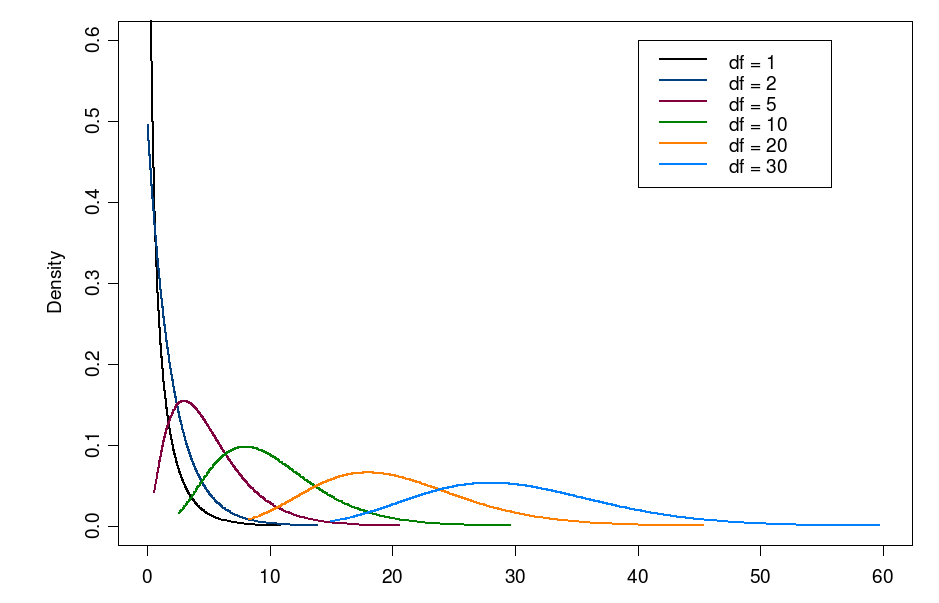
\includegraphics[scale=0.33]{2_37.png}
  \end{figure}
\end{frame}

\livelloB{Student's t-distribution}

\begin{frame}
  \vspace*{.3cm}
  The \textbf{Student's t}-distribution takes into consideration the relations among the mean and the variance estimations, \textbf{in little size samples}, when the sample variance is used.\\
  \vspace*{.3cm}
  The choice between the use of the normal distribution and the Student's t-distribution in the comparison among means comes from the knowledge of the $ \sigma^2 $ variance of the population or from the fact that it is unknown. In this last case, it is necessary to use the $ s^2 $ sample variance.\\
  \vspace*{.3cm}
  The Student's t random variable is defined as the ratio between a standard normal random variable and the square root of a $ \chi^2 $ divided by its degrees of freedom:
  $$ t_\nu = \frac{Z}{\sqrt{\chi^2_\nu/\nu}} $$
\end{frame}

\begin{frame}
  If a series of $ n $ observations ($ X_1, \cdots , X_n $) is drawn by a normal distribution, it is possible to show that the ratio
  \vspace*{.2cm}
  $$t_{n-1}=\frac{\overline{X}-\mu}{s/\sqrt{n}}$$\\
  \vspace*{.2cm}
  is distributed as a Student's t with $ n - 1 $ degrees of freedom. \\
  \vspace*{.5cm}
  \textbf{The corresponding curve is defined between $-\infty$ and $+\infty$, symmetric, little lowly that the normal and with higher frequencies in the extremes, when the number of df ({\boldmath $ \nu $}) is really small.}\\
  \vspace*{.5cm}
  Starting from a number of degrees of freedom around 30, the Student's t-distribution tends to a normal distribution.
\end{frame}

\begin{frame}
  \vspace*{.5cm}
  \centering
  This is a graphical representation of a Student's t distribution:\\
  \begin{figure}
    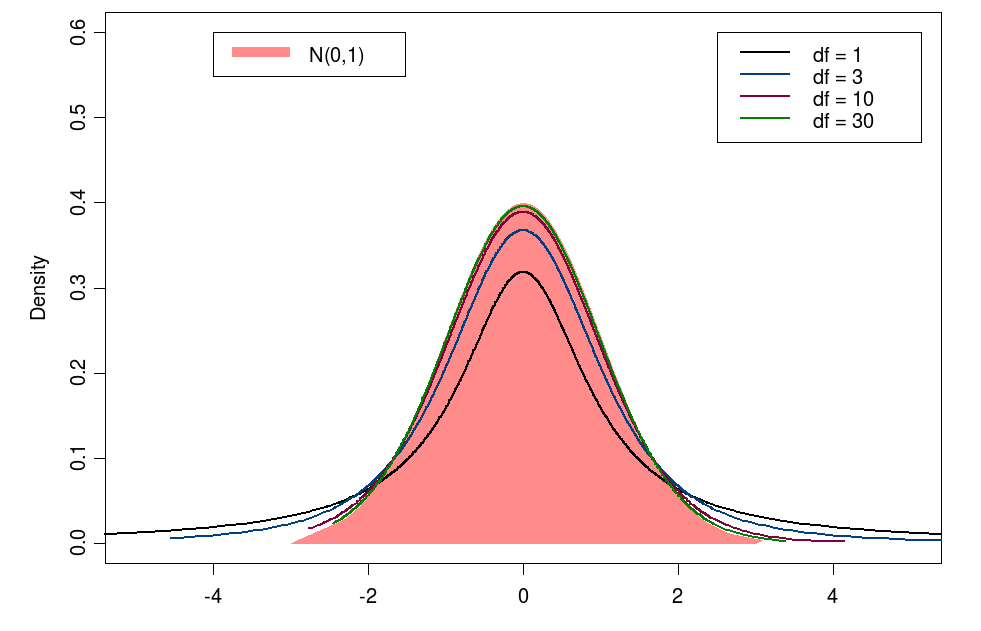
\includegraphics[scale=0.33]{2_40.png}
  \end{figure}
\end{frame}

\livelloB{F-distribution}

\begin{frame}
  Another interesting distribution, from which it is founded the inference of a big part of the parametric statistics, is the \textbf{F-distribution}.\\
  \vspace*{.2cm}
  It corresponds to the distribution of the \textbf{ratio of 2 chi-squared indipendent random variables} ($ A $ e $ B $), \textbf{divided by its corresponding degrees of freedom} ($ m $ e $ n $).\\
  \vspace*{.2cm}
  This \textbf{ratio F is defined between 0 and {\boldmath $ +\infty $}.}\\
  \vspace*{.2cm}
  The F distribution represents a \textbf{generalization} of the t distribution.\\
  \vspace*{.2cm}
  The t and $ \chi^2 $ distribution have only one parameter, the F has \textbf{two parameters}: the number of degrees of freedom both of the numerator and of the denominator.\\
  \vspace*{.2cm}
  \textbf{The square of a random variable t of Student with n degrees of freedom is equal to a F of Fisher distribution with degrees of freedom {\boldmath $ 1 $} and {\boldmath $ n $}.}
\end{frame}

\begin{frame}
\vspace*{.5cm}
\centering
This is the graphical representation of a F-distribution\\
\begin{figure}
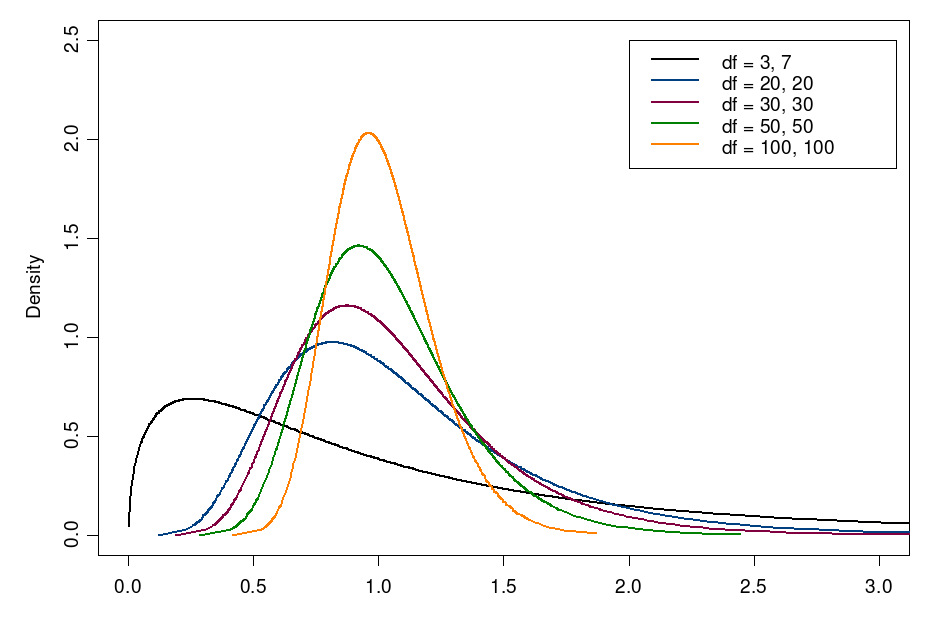
\includegraphics[scale=0.33]{2_42.png}
\end{figure}
\end{frame}

\livelloB{Lognormal distribution}

\begin{frame}
  \vspace*{.25cm}
  A distribution which is highly used in the risk analysis and for extreme events, is the \textbf{lognormal distribution}. \\
  \vspace*{.35cm}
  $$ y = f(x; \mu, \sigma) = \frac{1}{x\sigma\sqrt{2\pi}}\cdot exp\left\{-\frac{(log(x)-\mu)^2}{2\cdot \sigma^2}\right\} $$ \\
  \vspace*{.35cm}
  It corresponds to normal data distribution transformed by the exponential function. \\
  \vspace*{.35cm}
  That is: lognormal data transformed by a natural logarithm are distributed as a normal. Normal data transformed by the exponential are distributed as a lognormal.\\
  \vspace*{.35cm}
  The lognormal distribution \textbf{is defined between 0 and {\boldmath$+\infty$}}, extremes excluded. \\
\end{frame}

\begin{frame}
  The lognormal distribution mean is:
  $$ E[X] = e^{\mu + \sigma^2/2} $$
  The lognormal distribution variance is:
  $$ Var[X] = (e^{\sigma^2} - 1) e^{2 \mu + \sigma^2}$$\\
  Using the lognormal distribution is quite difficult because the parameters have a big variability for little variations of a right tale. In order to modify the right ``tale'' 's behavior of the lognormal distribution, it is often necessary a big variation of the parameters' values.\\
  This leads to an ``instability'' of the parameters' estimations (an ``high'' value more or less can lead to estimated parameters' values really different among them).
\end{frame}

\begin{frame}
  \vspace*{.5cm}
  \centering
  Graphical representation of the lognormal, when $ \sigma $ values change: \\
  \begin{figure}
    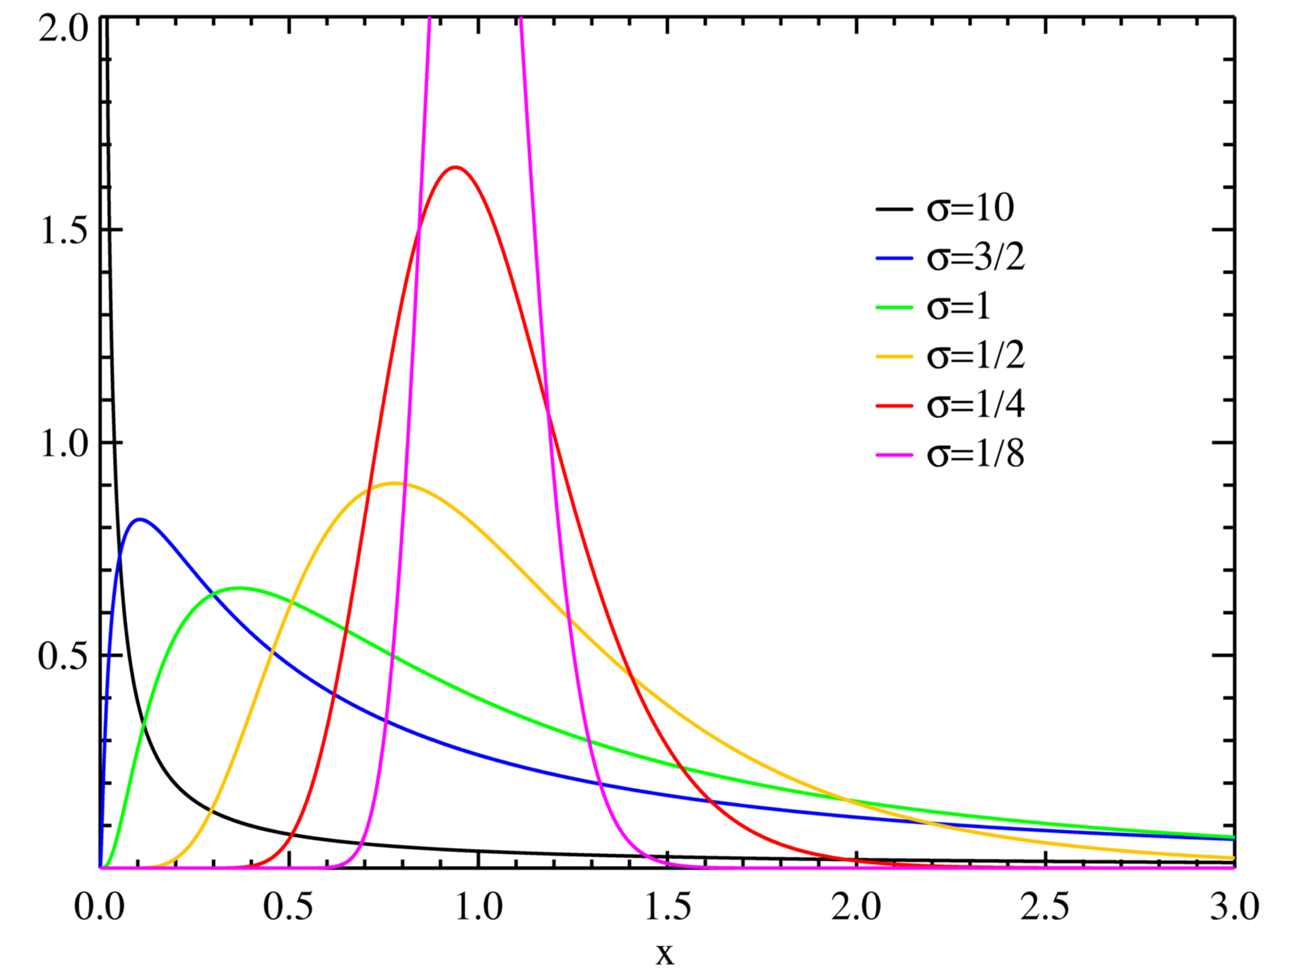
\includegraphics[scale=0.8]{LognormalDistribution.png}
  \end{figure}
\end{frame}

\livelloB{Weibull distribution}

\begin{frame}
  \vspace*{.5cm}
  The \textbf{Weibull distribution} is another distribution which is highly used in the risk analysis and for extreme events.\\
  \vspace*{.5cm}
  $$ y = f(x; \lambda, k) = \frac{k}{\lambda}\left( \frac{x}{\lambda}\right)^{k-1} \cdot e^{-\left(\frac{x}{\lambda} \right)^{k-1}} $$ \\
  \vspace*{.75cm}
  Where $ k > 0 $ is called the \textbf{shape} parameter and $ \lambda > 0 $ is called the \textbf{scale} parameter. \\
  \vspace*{.75cm}
  The Weibull distribution \textbf{is defined between 0 (included) and {\boldmath $ +\infty $}.} \\
\end{frame}

\begin{frame}
  The Weibull distribution mean is:
  $$ E[X] = \lambda \Gamma \left( 1 + \frac{1}{k} \right) $$
  The Weibull distribution variance is:
  $$ Var[X] = \lambda^2 \Gamma \left( 1 + \frac{2}{k} \right) - \left[ \lambda \Gamma \left( 1 + \frac{1}{k} \right) \right]^2 $$ \\
  The Weibull distribution, as the lognormal one, is difficult to use because of its parameters' variability for little variations of the right tale. In order to modify the behavior of the right ``tail'' of the Weibull distribution, it is often necessary a big variation of the parameters' values. This leads to an ``instability'' of the parameters' estimations.
\end{frame}

\begin{frame}
  \vspace*{.5cm}
  \centering
  Graphical representation of the Weibull distribution, when $ k $ values change: \\
  \begin{figure}
    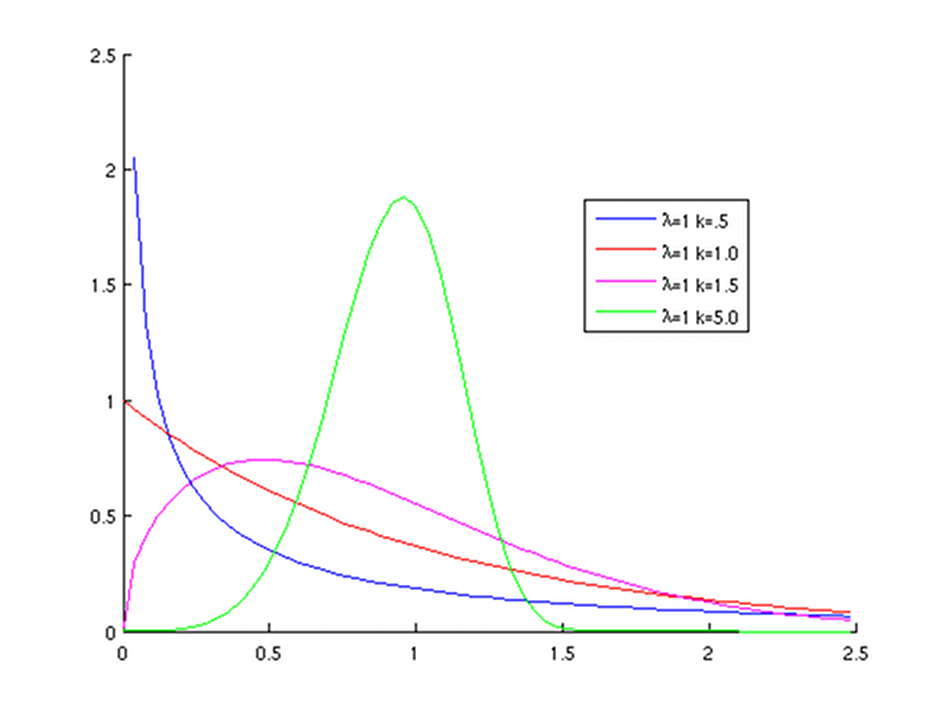
\includegraphics[scale=0.7]{WeibullDistr.png}
  \end{figure}
\end{frame}


